\chapter{插入图形}

图形是论文中描述实验结果及相关情况的一种重要方式,也是论文中经常使用的一种特殊信息语言。
一般来说,在科技论文中,通过正确地使用图形来辅助论文内容的理解与结果的表达,可以更直观地
展现论文内容,有助于得出正确结论。尤其在科研的数据分析中,能形直观地反映变量与变量之间的
关系,能清楚地表达某一变量的发展趋势等。很多时候图形能帮助读者领会文字难以表达的内容,同
样重要的是它往往可以起到减少篇幅、方便读者阅读的作用。许多图形是在做实验时用相应的软件生
成,在撰写论文时需要将其插入文档中,LaTeX可以较为方便地插入各种格式的图形。

本章将介绍如何在LaTeX中插入图形:
\begin{itemize}
    \item 首先在第1节中介绍如何以浮动体的形式插入图片,允许LaTeX根据内置的算法对图片位置进行调整;
    \item 第2节中介绍以非浮动体形式插入图片的环境命令;
    \item 第3节中介绍在文档中插入图目录、表目录的方式;
    \item 第4节中介绍对图表标题样式的调整方式;
    \item 第5节中介绍如何插入子图,并对子图的横纵向间距进行调整;
    \item 第6节中介绍图片的排列布局方式。
\end{itemize}

\section{插入浮动图片}

LaTeX中可以支持插入\emph{.pdf}、\emph{.jpg}、\emph{.jpeg}、\emph{.png}、\emph{*.eps}
等常见格式的图片,而对于LaTeX不支持的图片文件格式,如SVG格式的矢量图,则需要先转换再插入。
一般而言,读者可以通过截图、MS Visio等绘图工具、或者Matlab等编程工具制作并导出目标图片。

在LaTeX中插入图片可以使用\emph{graphicx}宏包,该宏包提供的\texttt{\textbackslash{}includegraphics[参数]\{文件名或文件路径\}}命令可以用于插入图片,以及设置参数以调整图片样式,常用参数包括:
\begin{itemize}
    \item width:设置图片宽度;
    \item height:设置图片高;
    \item scale:设置图片的缩放倍数;
    \item angle:设置图片的顺时针旋转角度(负值表示逆时针旋转)等。
\end{itemize}

一般而言,对于参数height和width,只需要调整其中一个即可,另一个参数将根据图片比例进行自动
缩放。而如果同时调整了参数height和width(不推荐),可能会改变图片比例,导致图片变形。

\emph{【例】}在导言区使用\texttt{\textbackslash{}usepackage\{graphicx\}}声明语句,
在主体代码中使用\texttt{\textbackslash{}includegraphics}命令插入图片,并调整图片样式参数:
\begin{lstlisting}[language=TeX]
    \usepackage{graphicx}
    \begin{document}

    The following figure shows a beautiful butterfly.

    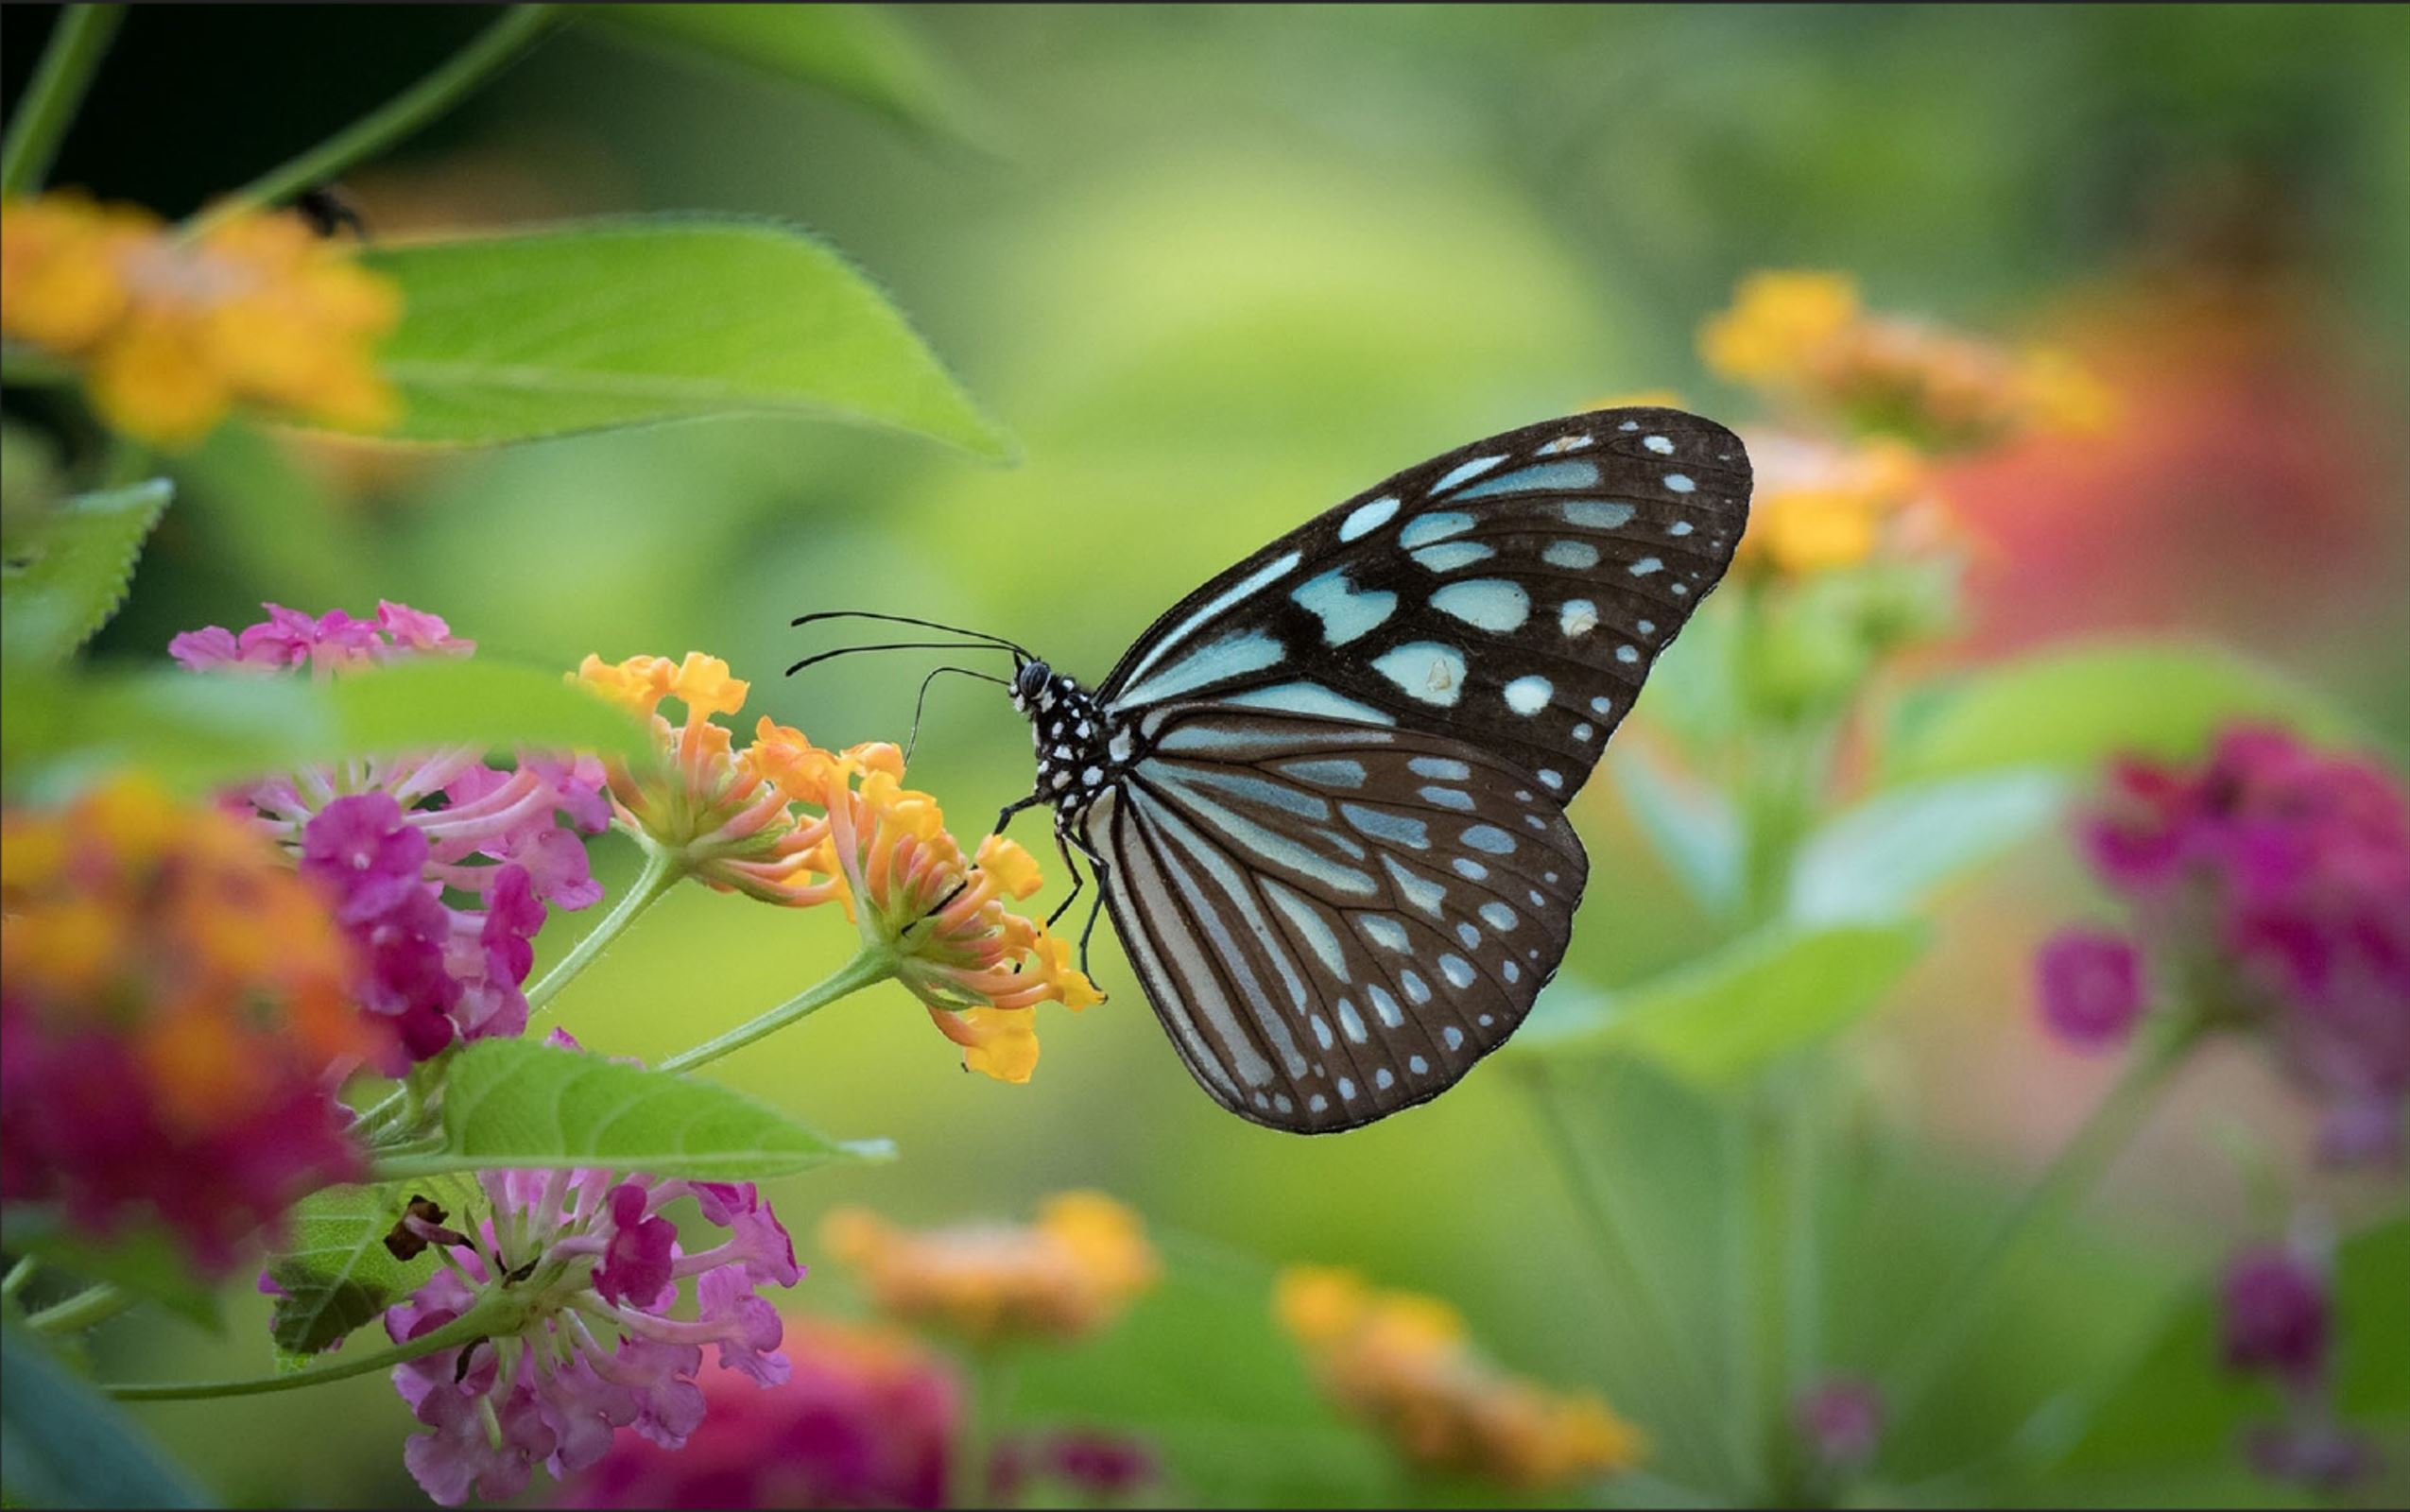
\includegraphics[width = 0.5\textwidth]{butterfly.JPG} % 插入第一张图片

    \vspace{12pt}

    Rotate the figure by 90 degrees.

    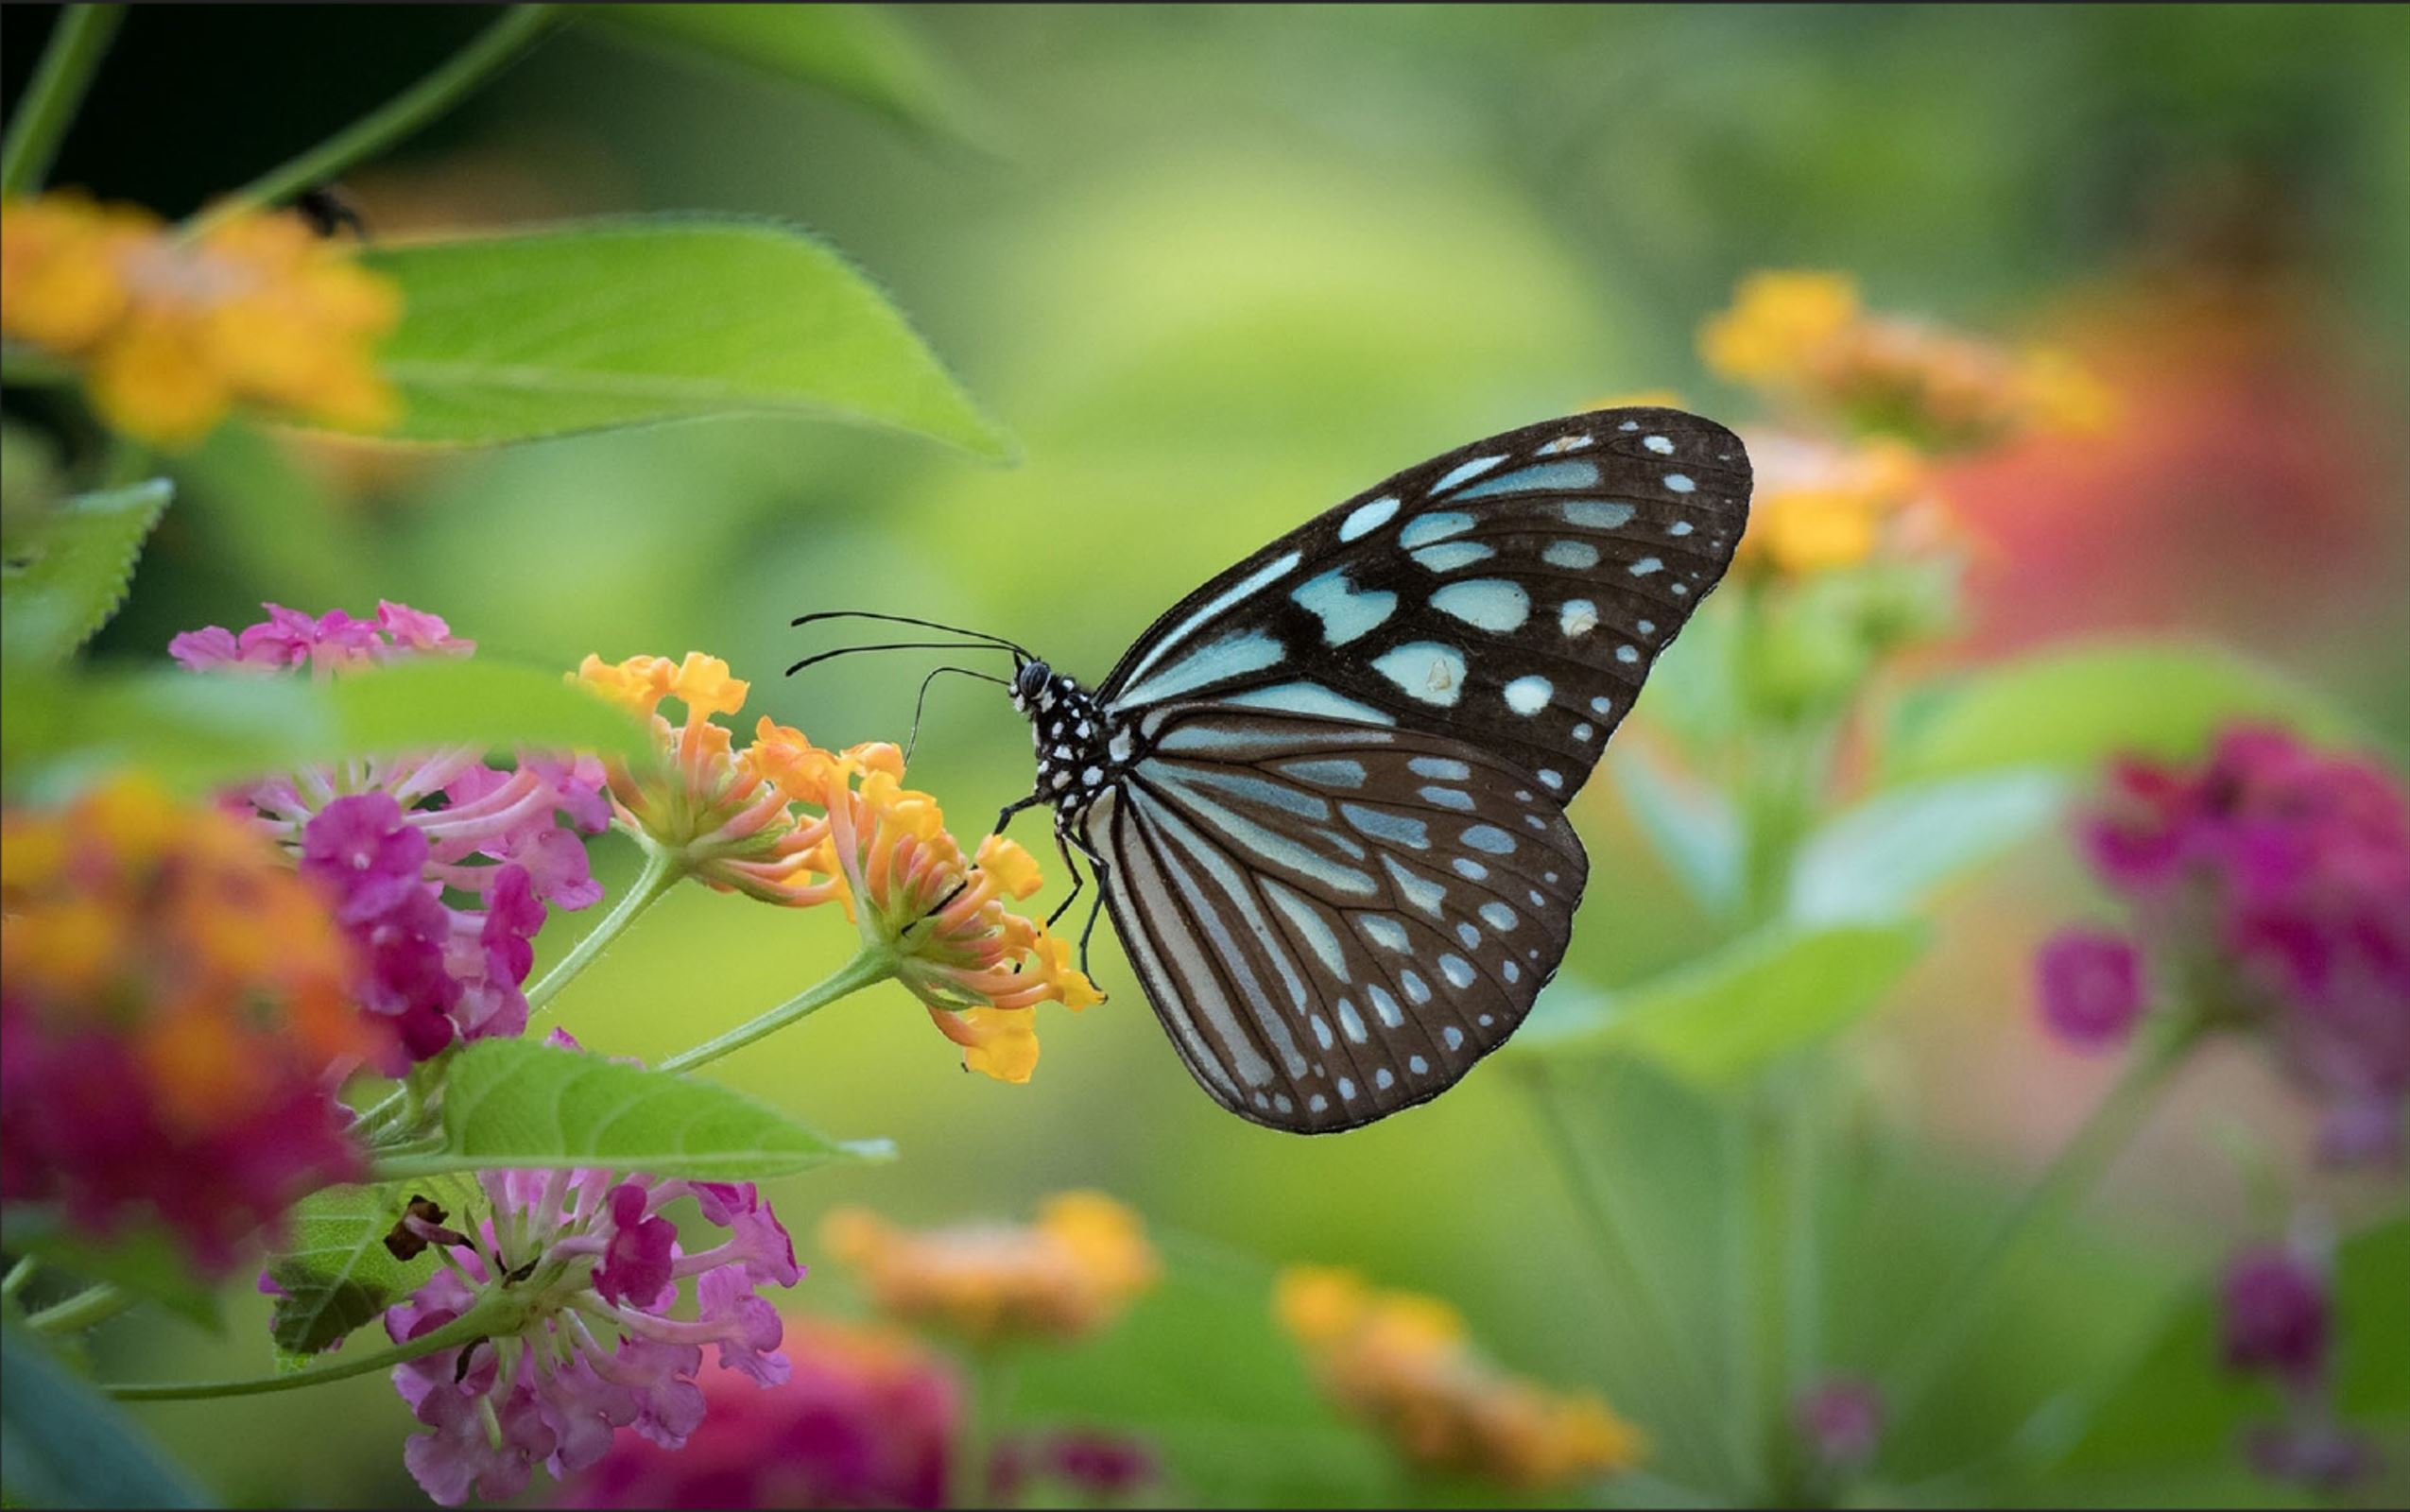
\includegraphics[width = 0.5\textwidth,angle = 90]{butterfly.JPG} % 插入第二张图片
\end{lstlisting}

此外,graphicx宏包提供了\emph{figure}环境语句,通过嵌套\texttt{\textbackslash{}includegraphics}
命令可以以浮动体的形式插入图片,从而能够实现自动递增编号、设置位置控制参数、利用\texttt{\textbackslash{}caption}
命令创建标题名称等。

\emph{【例】}使用figure环境嵌套\texttt{\textbackslash{}includegraphics}命令插入浮动
图片,并使用\texttt{\textbackslash{}label}命令为图片创建索引标签,然后在文本内容中使用
\texttt{\textbackslash{}ref}命令引用该图片:
\begin{lstlisting}[language=TeX]
    \usepackage{graphicx}
    \begin{document}

    Figure \ref{fig:1} shows a beautiful butterfly.

    \begin{figure}[htbp]
    \centering
        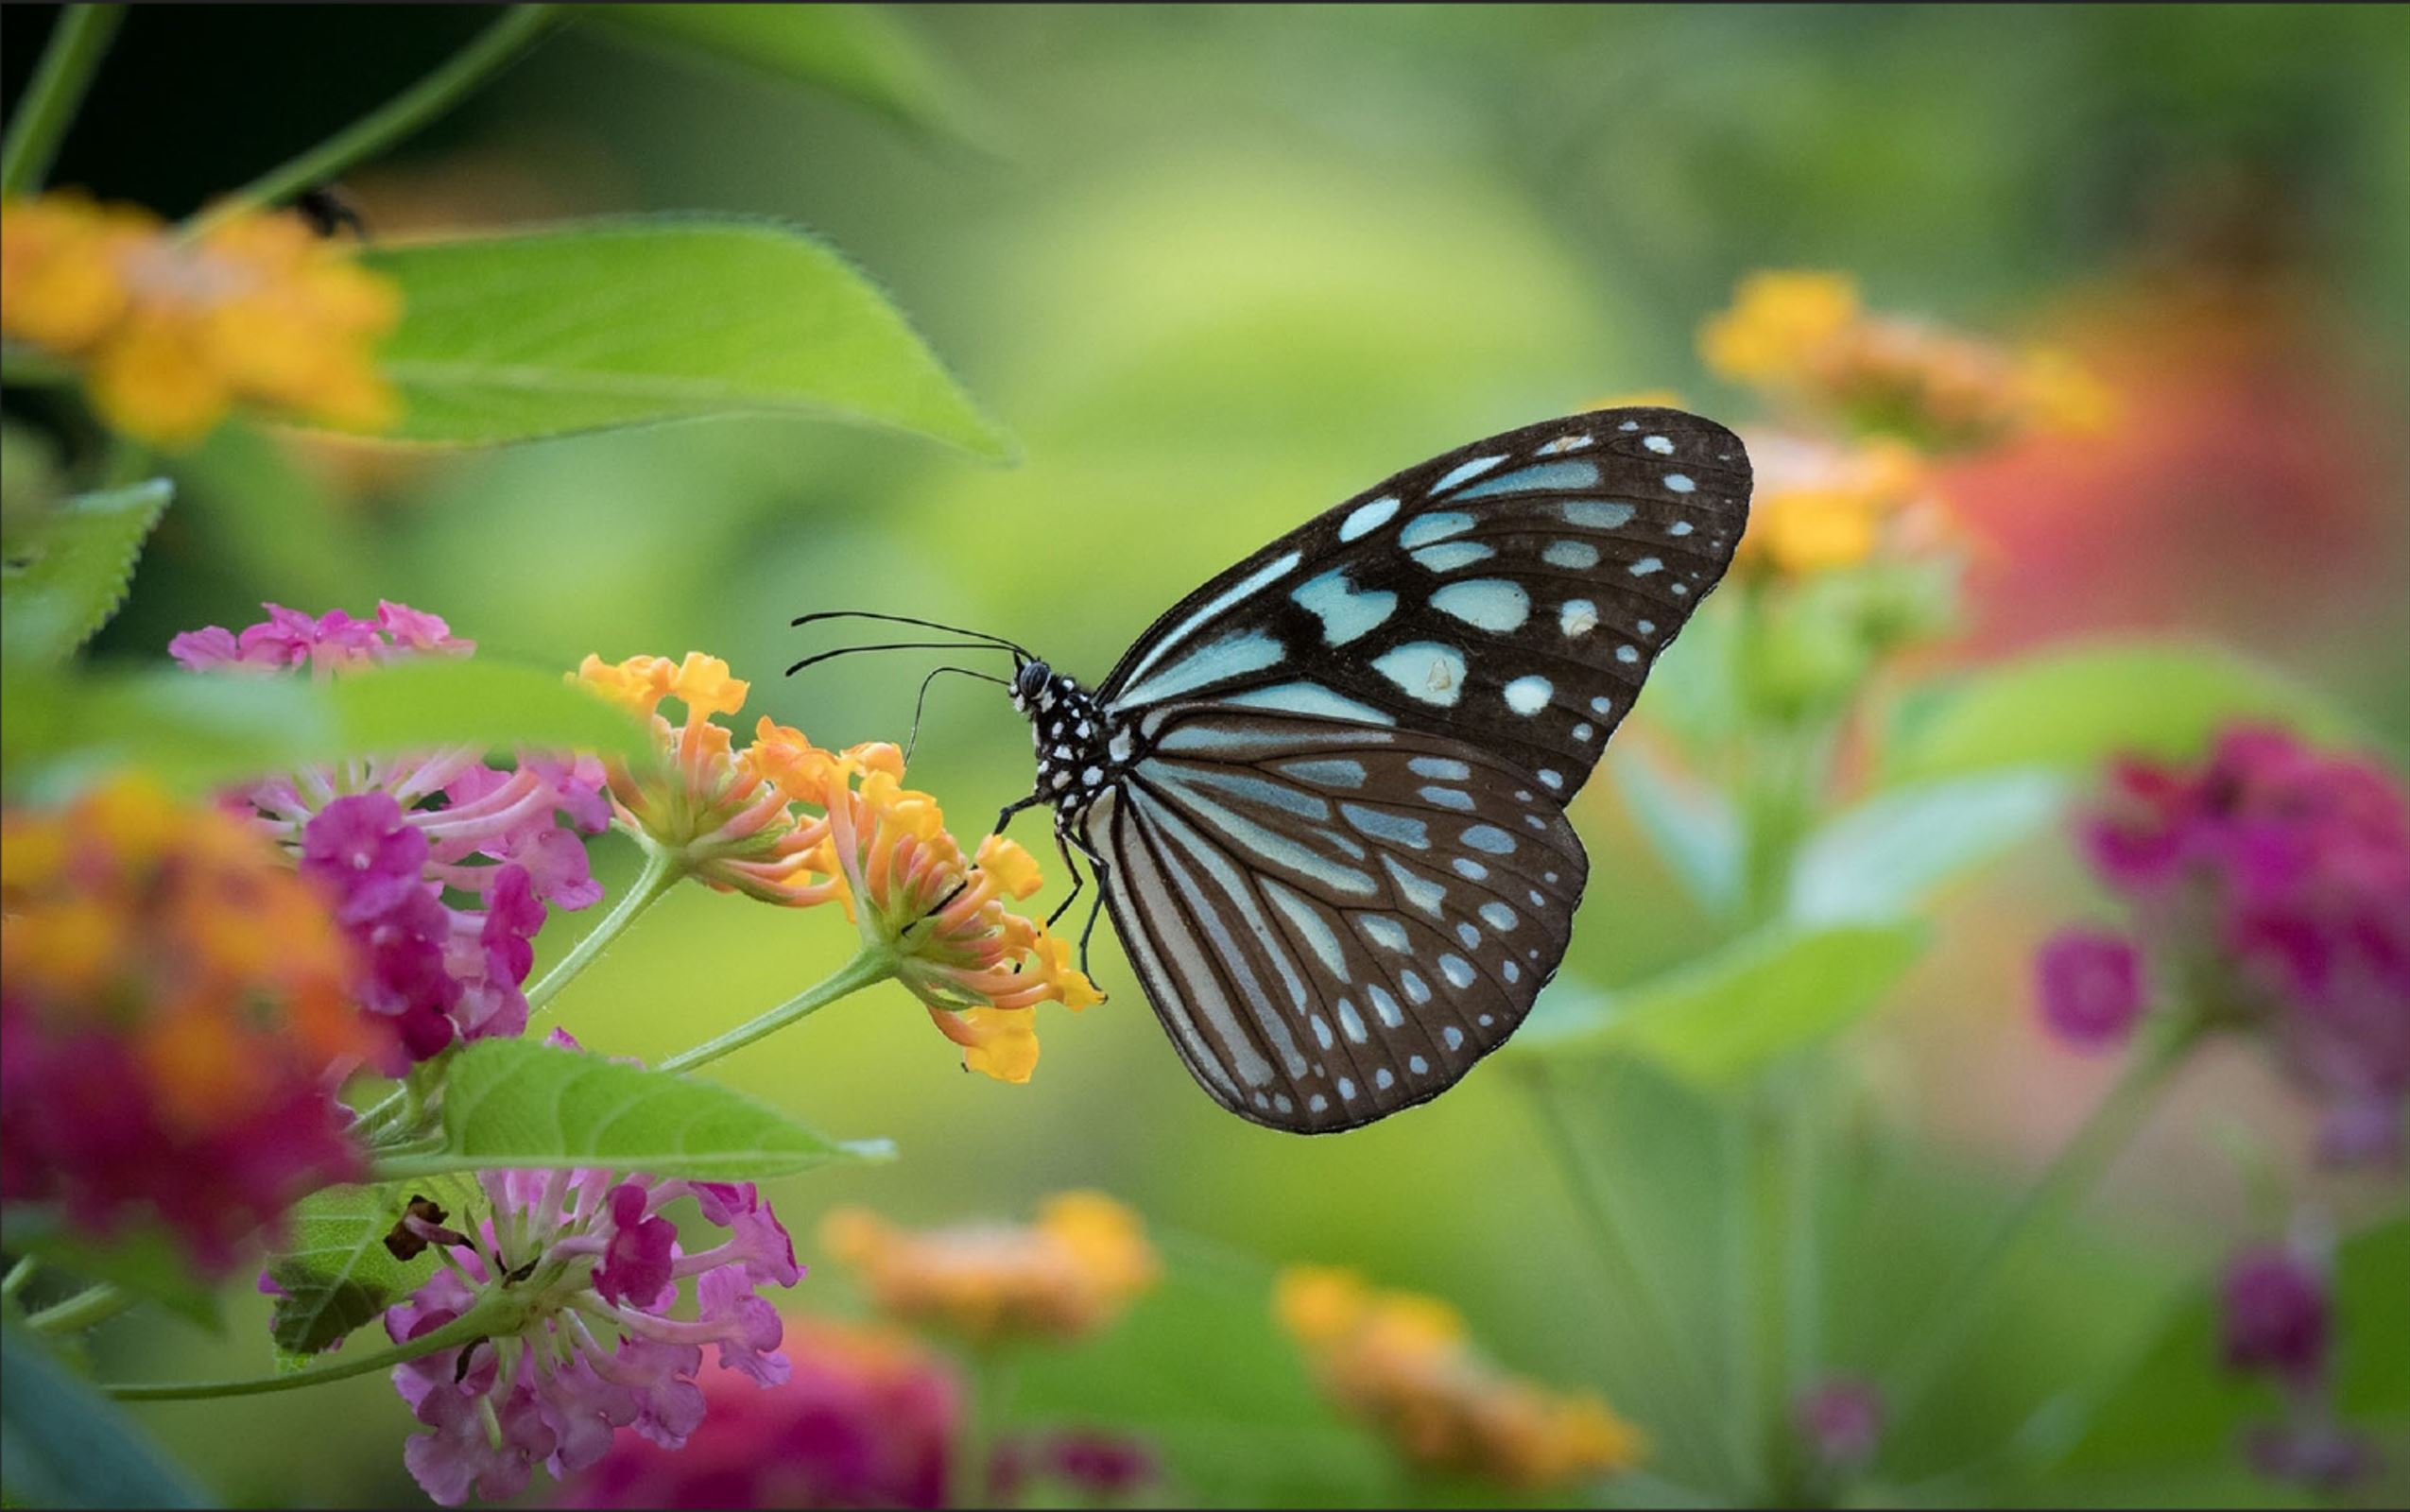
\includegraphics[width = 0.8\textwidth]{butterfly.JPG}
        \caption{A beautiful butterfly.}
        \label{fig:1}
    \end{figure}
\end{lstlisting}

如果想要创建取消编号的标题,则应调用\emph{caption}宏包、并使用\texttt{\textbackslash{}caption*}
命令创建标题名称。此时,LaTeX内置的自动编号计数器将暂停,直到遇到下一个\texttt{\textbackslash{}caption}
命令才会继续递增计数,例如:
\begin{lstlisting}[language=TeX]
    \caption{The first figure.} % 创建标题“Figure 1:  The first figure.”
    \caption*{The second figure.} % 创建标题“The second figure.”
    \caption{The third figure.} % 创建标题“Figure 2:  The third figure.”
\end{lstlisting}